% This file is part of MUST (Marmot Umpire Scalable Tool)
%
% Copyright (C)
%   2010-2016 ZIH, Technische Universitaet Dresden, Federal Republic of Germany
%   2010-2018 Lawrence Livermore National Laboratories, United States of America
%   2013-2018 RWTH Aachen University, Federal Republic of Germany
%
% See the LICENSE file in the package base directory for details


% \documentclass[english]{article}
\documentclass[english]{scrartcl}
\usepackage[latin9]{inputenc}
\usepackage{fancyhdr}
\pagestyle{fancy}
\usepackage{array}
\usepackage{longtable}
\usepackage{varioref}
\usepackage{float}
\usepackage{fancybox}
\usepackage{calc}
\usepackage[usenames]{color}
\usepackage{graphicx}
\usepackage{subfigure}
\usepackage{setspace}
\usepackage{url}
\usepackage{babel}
\usepackage{listings}
\usepackage{colortbl}
\usepackage{xspace}
\usepackage{hyperref}

% P^nMPI
\DeclareMathAlphabet{\mathtr}{OT1}{cmr}{}{n}
\newcommand{\pnmpi}{$\mathop{\mathtr{P^nMPI}}\nolimits$\xspace}


\definecolor{LGREY}{rgb}{0.45,0.45,0.45}

\definecolor{MustBlue1}{rgb}{0.60,0.60,0.87}
\definecolor{MustBlue2}{rgb}{0.47,0.47,0.73}
\definecolor{MustRedDark}{rgb}{1,0.87,0.87}
\definecolor{MustRedLight}{rgb}{1,0.93,0.93}
\definecolor{MustRedDarkGray}{rgb}{0.93,0.80,0.80}
\definecolor{MustRedLightGray}{rgb}{0.93,0.87,0.87}

\emergencystretch = 0 pt
\pretolerance = 150
\tolerance = 10000
\hbadness = 9999
\hfuzz = 0 pt


% redefine paragraph to have a linebreak after it and let \emph work as well
\makeatletter
\renewcommand\paragraph{\@startsection{paragraph}{4}{\z@}%
  {-3.25ex\@plus -1ex \@minus -.2ex}%
  {1.5ex \@plus .2ex}%
  {\normalfont\normalsize\bfseries}}
\makeatother


\begin{document}

\title{\textsf{\textcolor{blue}{\Huge}}\\
\begin{center}
MUST
\end{center}
\textsf{\large MPI Runtime Error Detection Tool}\\
\vspace{8ex}
\centering
\includegraphics[width=0.55\textwidth]{logo.pdf}
}
\maketitle

\newpage{}

\tableofcontents{}

\newpage{}

\section{Introduction}

MUST detects usage errors of the Message Passing Interface (MPI) and reports
them to the user.
As MPI calls are complex and usage errors common, this functionality is
extremely helpful for application developers that want to develop correct MPI applications.
This includes errors that already manifest as segmentation faults or incorrect
results, as well as many errors that are not visible to the application
developer or do not manifest on a certain system or MPI implementation. 

To detect errors, MUST intercepts the MPI calls that are issued by the target
application and evaluates their arguments. The two main usage
scenarios for MUST arise during application development and during porting.
When a developer adds new MPI communication calls, MUST can detect
newly introduced errors, especially  also some that may not manifest in an
application crash. Further,
before porting an application to a new system, MUST can detect violations to the
MPI standard that might manifest on the target system. MUST reports errors
in a log file that can be investigated once the execution of the target
executable finishes (irrespective of whether the application crashed or not).

\section{Installation}

The MUST software consists of three individual packages:
\begin{itemize}
  \item \pnmpi
  \item GTI
  \item MUST
\end{itemize}

The \pnmpi package provides base infrastructure for the MUST software and
intercepts MPI calls of the target application. GTI provides tool
infrastructure, while the MUST package contains the actual correctness checks.

Starting with 1.6, all three packages are contained in a single archive and
configured and built at once.

Each MUST installation is built with a certain compiler and MPI library. It
should only be used for applications that are built with the same pair of
compiler and MPI library. This is necessary as the behavior of MUST may differ
depending on the MPI library. Compilers may be mixed if they are binary
compatible.

Building must requires CMake for configuration, it is freely available at
\url{http://www.cmake.org/}. You can execute \emph{which cmake} to determine
whether a CMake installation is available. If not, contact your system
administrator or install a local version, which requires no root
privileges. We suggest to use CMake version 3.9 or later 
(use \emph{cmake \mbox{-{}-}version}) for full functionality.

Further, in order to augment the MUST output with call stack information, which
is very helpful for pinpointing errors, it is possible to utilize Dyninst. In
that case MUST uses the Stackwalker API from Dyninst to read and print
stacktraces for errors. As the installation of Dyninst is often non-trivial we
suggest this for more experienced users or administrators only.
Section~\ref{section:dyninst} presents the necessary steps for such an
installation.

MUST supports parallel build, therefore you may want
to append \emph{\mbox{--}j\textless number of cores\textgreater} to the make
calls.

\subsection{Prerequisites to build and use MUST}
\begin{itemize}
 \item cmake (required 3.9 or newer, see \emph{cmake \mbox{-{}-version}})
 \item python (required 2.6 or newer, see \emph{python \mbox{-V}})
 \item libxml2 with headers (libxml2-dev / libxml2-devel, required)
 \item graphviz (optional, to generate graphs)
 \item dyninst (optional, see section \ref{section:dyninst})
 \item a browser (optional, to view html output)
 \item MPI library, used by the application (required)
\end{itemize}
\subsection{Configuring with CMake}
All parts of MUST use CMake for configuration.
CMake works best with 'out of source' builds, this is what we recommend in
the installation steps below. 
Common CMake options include \verb|-DCMAKE_INSTALL_PREFIX| to set the path to
install to, if you do not have root or to create module environment packages.
CMake options can be configured with a GUI on many systems by using
\verb|ccmake| instead of cmake with all the -D flags listed below.
\begin{itemize}
     \item When the ccmake gui appears:
     \item press c to generate options, press e to move on from any messages displayed by cmake. 
     \item edit any options displayed, 
     \item press c to see if there are any new options resulting from the previous round of choices
     \item repeat until you are happy with the options
     \item press g to generate the build
     \item  move on to the make step as usual.
\end{itemize}
\subsection{Building MUST}
MUST can be build as follows (assuming GNU compilers):
\begin{verbatim}
tar xzf MUST-v1.6-rc1.tar.gz
cd MUST-v1.6-rc1
mkdir BUILD
cd BUILD
CC=$(which gcc) CXX=$(which gcc++) FC=$(which gfortran) \
cmake ../ \
     -DCMAKE_INSTALL_PREFIX=<MUST-INSTALLATION-DIR> \
     -DCMAKE_BUILD_TYPE=Release
make -j8 install
export PATH=<MUST-INSTALLATION-DIR>/bin:$PATH
\end{verbatim}

In many cases it's essential, to use the plain compilers for \emph{CC}\&Co, i.e., not
the MPI compiler wrappers.
The CMake call will determine your MPI installation in order to configure
MUST correctly. If this should fail -- or multiple MPIs are available -- you
can tip the configuration by specifying
\emph{\mbox{--}DMPI\_C\_COMPLIER=$<$FILE\mbox{--}PATH\mbox{--}TO\mbox{--}MPICC$>$} as well as
\emph{\mbox{--}DMPI\_CXX\_COMPLIER=$<$FILE\mbox{--}PATH\mbox{--}TO\mbox{--}MPICXX$>$} and
\emph{\mbox{--}DMPI\_Fortran\_COMPLIER=$<$FILE\mbox{--}PATH\mbox{--}TO\mbox{--}MPIF90$>$} as additional
arguments to the \emph{cmake} command. More advanced users can fine tune the
detection by specifying additional variables, consult the comments in
\emph{cmakemodules/FindMPI.cmake}. On clusters with special MPI-environments, it helps to 
verify that \emph{MPIEXEC} is set to the right mpiexec command (like srun).

Usually no extra arguments are needed to configure MUST. You can specify
\emph{-DENABLE\_TESTS=On} to activate the test suite that is included in MUST.
Tests should only be started after installing MUST and can be run with:
\begin{verbatim}
ctest
\end{verbatim}
Some tests will fail even for a correct installation since they document
future extensions. You can get a detailed test report for a single test with:
\begin{verbatim}
ctest -VV -R ^<TEST-NAME>$
\end{verbatim}
For the test named \emph{basic}:
\begin{verbatim}
ctest -VV -R ^basic$
\end{verbatim}

\subsection{Install Prebuilt Configurations}
To speed up the tool preparation time, we provide some prebuilt
configurations for typical tool usage. These can be installed during
building of MUST:
\begin{verbatim}
make -j8 install install-prebuilds
\end{verbatim}
We strongly suggest this step for cluster installations.
If prebuilts are not available, MUST will prepare an appropriate
configuration during the execution of mustrun.

\subsection{Environmentals}
To work with MUST, it is sufficient to add \emph{$<$MUST\mbox{--}INSTALLATION\mbox{--}DIR$>$/bin} 
to your \emph{PATH} variable. 

\section{Usage}

The following two steps allow you to use MUST:
\begin{itemize}
\item Replace the \emph{mpiexec} command with
\emph{mustrun} to execute your application;
\item Inspect the result file of the run.
\end{itemize}

\subsection{Execution}

The actual execution of an application with MUST is done by replacing the
\emph{mpiexec} command with \emph{mustrun}. It performs a code generation step
to adapt the MUST tool to your application and will run your application with
MUST afterwards. 

The plain \emph{mustrun} command that we use here is intended for small scale
short running applications and can exhibit very high runtime overhead.
Section~\ref{section:must-modes} presents further configurations of MUST that
we tested with up to $16,384$ processes.  The plain \emph{mustrun} command uses
all of MUST's correctness checks and a communication system where one MPI 
process is used to drive some of these
checks. So when submitting a batch job,
you should make sure to allocate resources for one additional task. Further,
when calling \emph{mustrun} you need to have access to the compilers and MPI
utilities that where used to build MUST itself.

A regular \emph{mpiexec} command like:
\begin{verbatim}
mpiexec -np 4 application.exe
\end{verbatim}
Is replaced with:
\begin{verbatim}
mustrun -np 4 application.exe
\end{verbatim}
It will execute your application with 4 tasks, but requires one additional task,
i.e. it will actually invoke \emph{mpiexec} with \emph{\mbox{-np 5}}.

For an example where the \emph{mpiexec} command and the switch used to
specify the number of process is named differently:
\begin{verbatim}
srun -n 4 application.exe
\end{verbatim}
You could use the following\emph{mustrun} command:
\begin{verbatim}
mustrun --must:mpiexec srun --must:np -n  -n 4 application.exe
\end{verbatim}

\noindent{}If your machine provides no compilers in batch jobs, you can prepare
a run as follows:
\begin{verbatim}
mustrun --must:mode prepare -np 4 application.exe
\end{verbatim}
In your batch job you would then just execute:
\begin{verbatim}
mustrun --must:mode run -np 4 application.exe
\end{verbatim}

\noindent{}The \emph{mustrun} tool provides further switches to modify its
behavior, call \mbox{\emph{mustrun \mbox{-{}-must:help}}} for a summary.  
If you
encounter errors during execution, please submit error reports where you use \emph{\mbox{-{}-must:verbose}} as
an argument to \emph{mustrun}.

\subsection{Execution of threaded applications}
For support of threaded applications, MUST provides a thread-safe mode:
\begin{verbatim}
mustrun --must:hybrid -np 4 application.exe
\end{verbatim}
Be aware, that MUST lifts the required MPI threading level in this case to
\texttt{MPI\_THREAD\_MULTIPLE}, while MUST limits the provided threading level without
this flag to \texttt{MPI\_THREAD\_SINGLE}.

\subsection{Results}
MUST stores its results in an HTML file named \emph{MUST\_Output.html}. It
contains information on all detected issues including information on where the
error occurred.

\section{Example}
As an example consider the following application that contains three MPI usage
errors:

\begin{lstlisting}[tabsize=3,numbers=none,basicstyle=\scriptsize,%
	breaklines=true,language=C, frame=single,%
	commentstyle=\color{LGREY}, keywordstyle=\bfseries,%
	identifierstyle=\bfseries, numbers=left, numbersep=5pt,numberstyle=\tiny,%
	name=example-interface-listing, firstnumber=1]
#include <stdio.h>
#include <mpi.h>

int main (int argc, char** argv)
{
    int rank,
        size,
        sBuf[2] = {1,2},
        rBuf[2];
    MPI_Status status;
    MPI_Datatype newType;

    MPI_Init(&argc,&argv);
    MPI_Comm_rank (MPI_COMM_WORLD, &rank);
    MPI_Comm_size (MPI_COMM_WORLD, &size);

    //Enough tasks ?
    	if (size < 2)
    	{
    		printf ("This test needs at least 2 processes!\n");
    		MPI_Finalize();
    		return 1;
    	}

    	//Say hello
    	printf ("Hello, I am rank %d of %d processes.\n", rank, size);

    	//1) Create a datatype
    	MPI_Type_contiguous (2, MPI_INT, &newType);
    	MPI_Type_commit (&newType);

    	//2) Use MPI_Sendrecv to perform a ring communication
    	MPI_Sendrecv (
    	        sBuf, 1, newType, (rank+1)%size, 123,
    	        rBuf, sizeof(int)*2, MPI_BYTE, (rank-1+size) % size, 123,
    	        MPI_COMM_WORLD, &status);

    	//3) Use MPI_Send and MPI_Recv to perform a ring communication
    	MPI_Send (sBuf, 1, newType, (rank+1)%size, 456, MPI_COMM_WORLD);
    	MPI_Recv (rBuf, sizeof(int)*2, MPI_BYTE, (rank-1+size) % size, 456, MPI_COMM_WORLD, &status);

    	//Say bye bye
    	printf ("Signing off, rank %d.\n", rank);

    MPI_Finalize ();

    return 0;
}
/*EOF*/
\end{lstlisting}

\subsection{Execution with MUST}

A user could set up the environment for MUST, build the application, and run
it with the following commands:

\begin{verbatim}
#Set up environment
export PATH=<MUST-INSTALLATION-DIR>/bin:$PATH

#Compile and link, we rely on the ld-preload mechanism
mpicc example.c -o example.exe -g

#Run with 4 processes, will need resources for 5 tasks!
mustrun -np 4 example.exe
\end{verbatim}

\subsection{Output File}

The output of the run with MUST will be stored in a file named
\emph{MUST\_Output.html}. For this application MUST will detect three different
errors that are:
\begin{itemize}
  \item A type mismatch (Figure~\ref{result-type})
  \item A send-send deadlock (Figure~\ref{result-deadlock} )
  \item A leaked datatype (Figure~\ref{result-leak} )   
\end{itemize}

\begin{figure}[t]
  \centering
  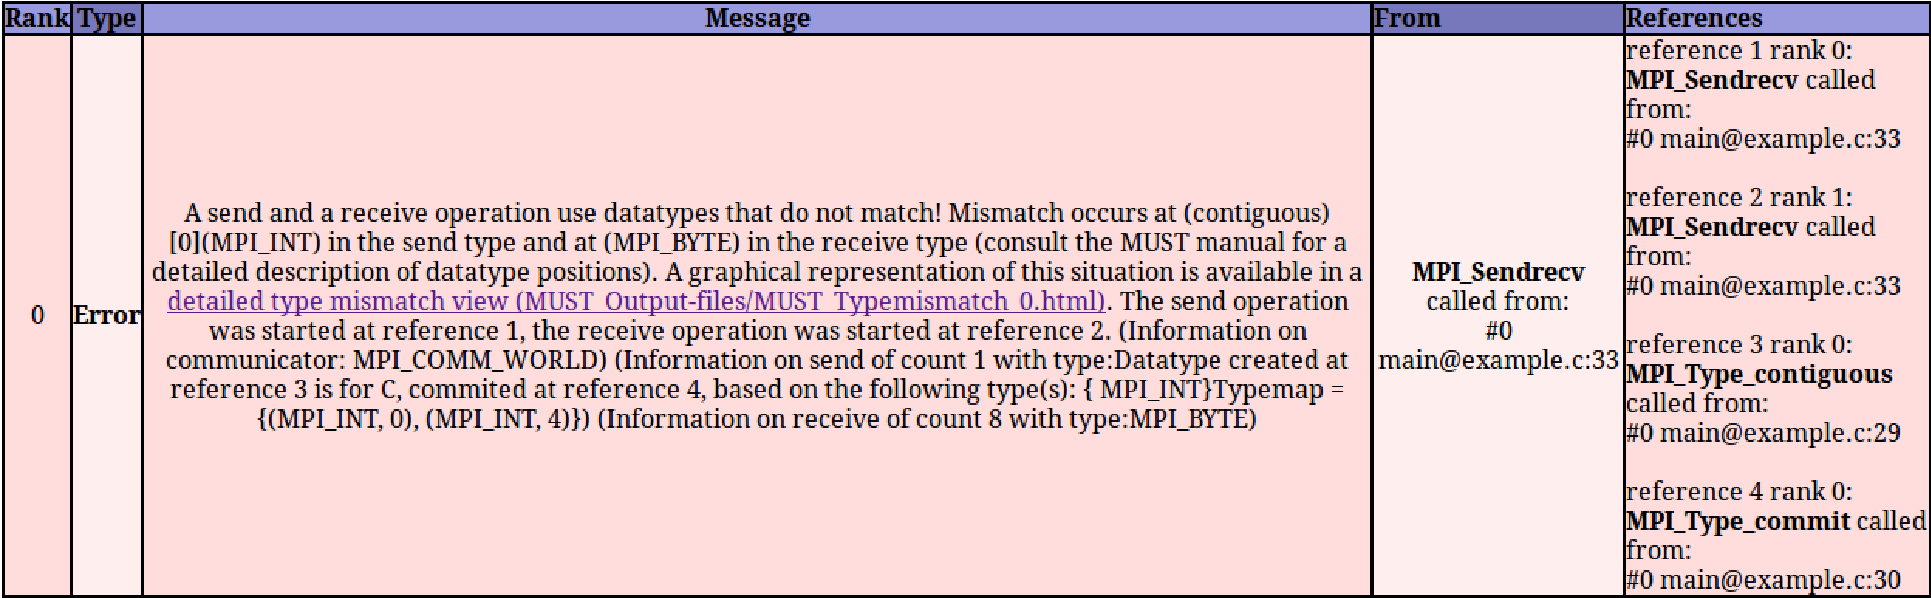
\includegraphics[angle=0,width=0.99\linewidth]{outputtypemismatch.pdf}
  \caption{Type mismatch error report from MUST.}
  \label{result-type}
  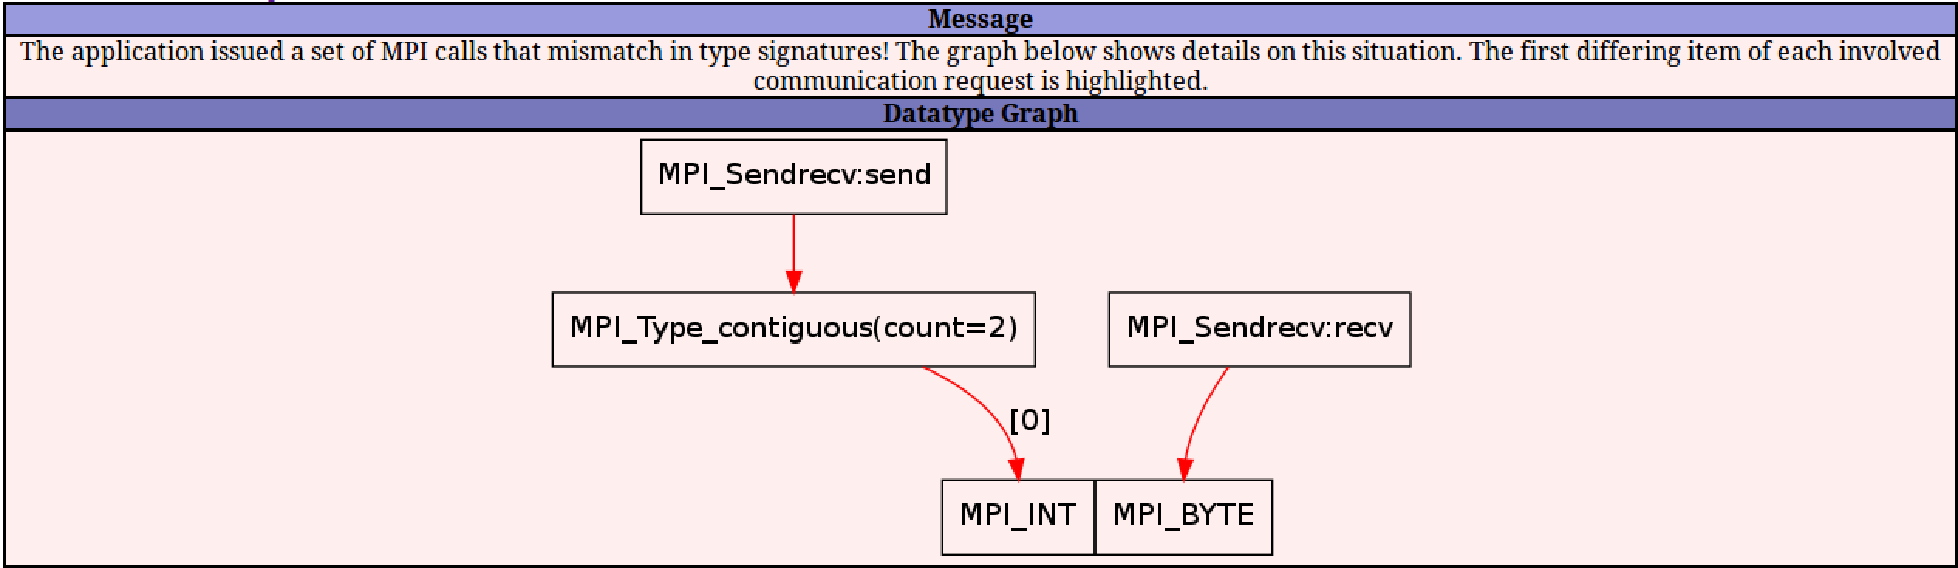
\includegraphics[angle=0,width=0.99\linewidth]{typemismatch.pdf}
  \caption{Detail page for the type mismatch in
  Figure~\ref{section:must-modes}.}
  \label{result-type-dot}
\end{figure}
% \begin{table}[hbtp]
% \begin{longtable}[t]{|m{0.05\textwidth}|m{0.06\textwidth}|m{0.38\textwidth}|m{0.14\textwidth}|m{0.23\textwidth}|}
% 
%     \multicolumn{5}{p{\textwidth}}{\textbf{MUST Output}, date: Thu Aug 25 09:04:01 2011.}\\\hline
%     \footnotesize\cellcolor{MustBlue1}\begin{center}\textbf{Rank} \end{center}&
%     \footnotesize\cellcolor{MustBlue2}\begin{center}\textbf{Type} \end{center}&
%     \footnotesize\cellcolor{MustBlue1}\begin{center}\textbf{Message} \end{center}&
%     \footnotesize\cellcolor{MustBlue2}\begin{center}\textbf{Form} \end{center}&
%     \footnotesize\cellcolor{MustBlue1}\begin{center}\textbf{References} \end{center}\\\hline
% 
% 
%     \footnotesize\cellcolor{MustRedDark}\begin{center}0\end{center} &
%     \footnotesize\cellcolor{MustRedLight}\begin{center}\textbf{Error}\end{center} &
%     \footnotesize\cellcolor{MustRedDark}\begin{center} A send and a receive
%     operation use datatypes that do not match! Mis-match occurs at (CONTIGUOUS)[0](MPI\_INT) in the send type and at (MPI\_BYTE) in the receive type (consult the MUST manual for a detailed description of datatype positions). The send operation was started at reference 1, the receive operation was started at reference 2. (Information on communicator: MPI\_COMM\_WORLD) (Informationon send of count 1 with type: Datatype created at reference 3 is for C, commited at reference 4, based on the following type(s): MPI\_INT) (Information on receive of count 8 with type:MPI\_BYTE)\end{center}& \footnotesize\cellcolor{MustRedLight}\begin{center}call MPI\_Sendrecv\end{center}&
%    \footnotesize\cellcolor{MustRedDark}\begin{center} reference 1: call\newline MPI\_Sendrecv @rank 3\newline
% reference 2: call\newline MPI\_Sendrecv @rank 0\newline
% reference 3: call\newline MPI\_Type\_contiguous @rank 3\newline
% reference 4: call\newline MPI\_Type\_commit @rank 3\end{center}\\
% \hline
% \end{longtable}
% \caption{Type mis-match error report from MUST.}
% \label{result-type}
% \centering
% \end{table}

Figure~\ref{result-type} shows the first error that MUST detects. The error
results from the usage of non-matching datatypes, which are an \texttt{MPI\_INT}
and an \texttt{MPI\_BYTE} of the same size as the integer value. This is not
allowed according to the MPI standard. A correct application would use
\texttt{MPI\_INT} for both the send and receive call.

If MUST is configured with Dyninst (Section~\ref{section:dyninst}), the right
column will list call stacks for all the involved MPI calls, as in
Figure~\ref{section:must-modes}. 
Here the 
error is detected in the \texttt{MPI\_Sendrecv} call in line 33.

The example shows the specification of the location in the datatype that causes
the mismatch. 
The location \texttt{(CONTIGUOUS)[0](MPI\_INT)} means that the used
datatype is of contiguous kind, the mismatch is within the first element of the
contiguous type which is defined to be a base type namely \texttt{MPI\_INT}.

As another example \texttt{(VECTOR)[1][2](MPI\_CHAR)} would address the third
entry of the second block of a vector with basetype \texttt{MPI\_CHAR}.

Figure~\ref{result-type-dot} displays a graphical representation of the type
mismatch. The image shows type trees of the involved datatypes. For a correct type match,
both trees should share all their leaves. For a clearer view, matching leaves
are hidden. The path to the first clash is highlighted in red.
For derived types, the node labels display the count/blocklength value, 
used in the 
declaration of the type, while the edge label (corresponding to the path expression) 
gives the index of the block/blockitem, that leads to the first clash. 

For communication buffers, that access the same memory address concurrently
("buffer overlap"), similar description and graphs are used. In this case all nodes that point 
to distinct memory addresses are hidden, as the focus lies on the
representation of the memory overlap.

\begin{figure}[tp]
  \centering
  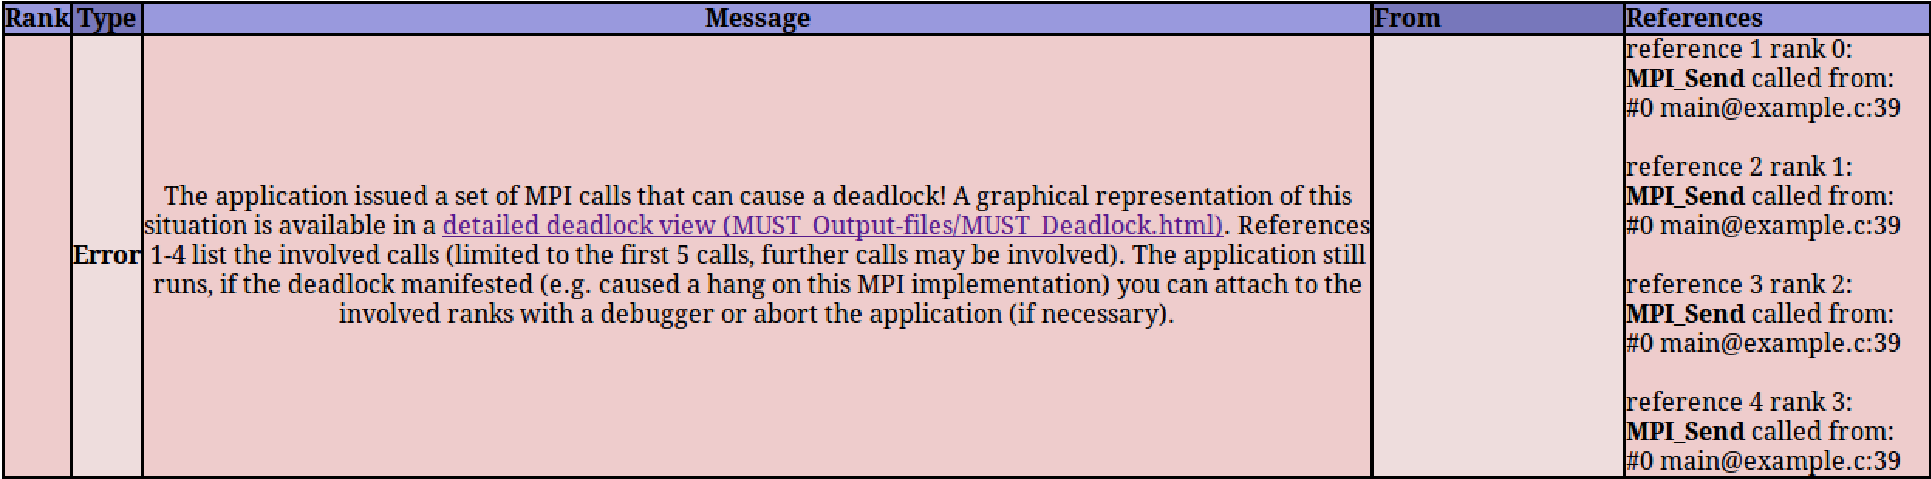
\includegraphics[angle=0,width=0.99\linewidth]{outputdeadlock.pdf}
  \caption{Send-send deadlock report from MUST, basic report.}
  \label{result-deadlock}
  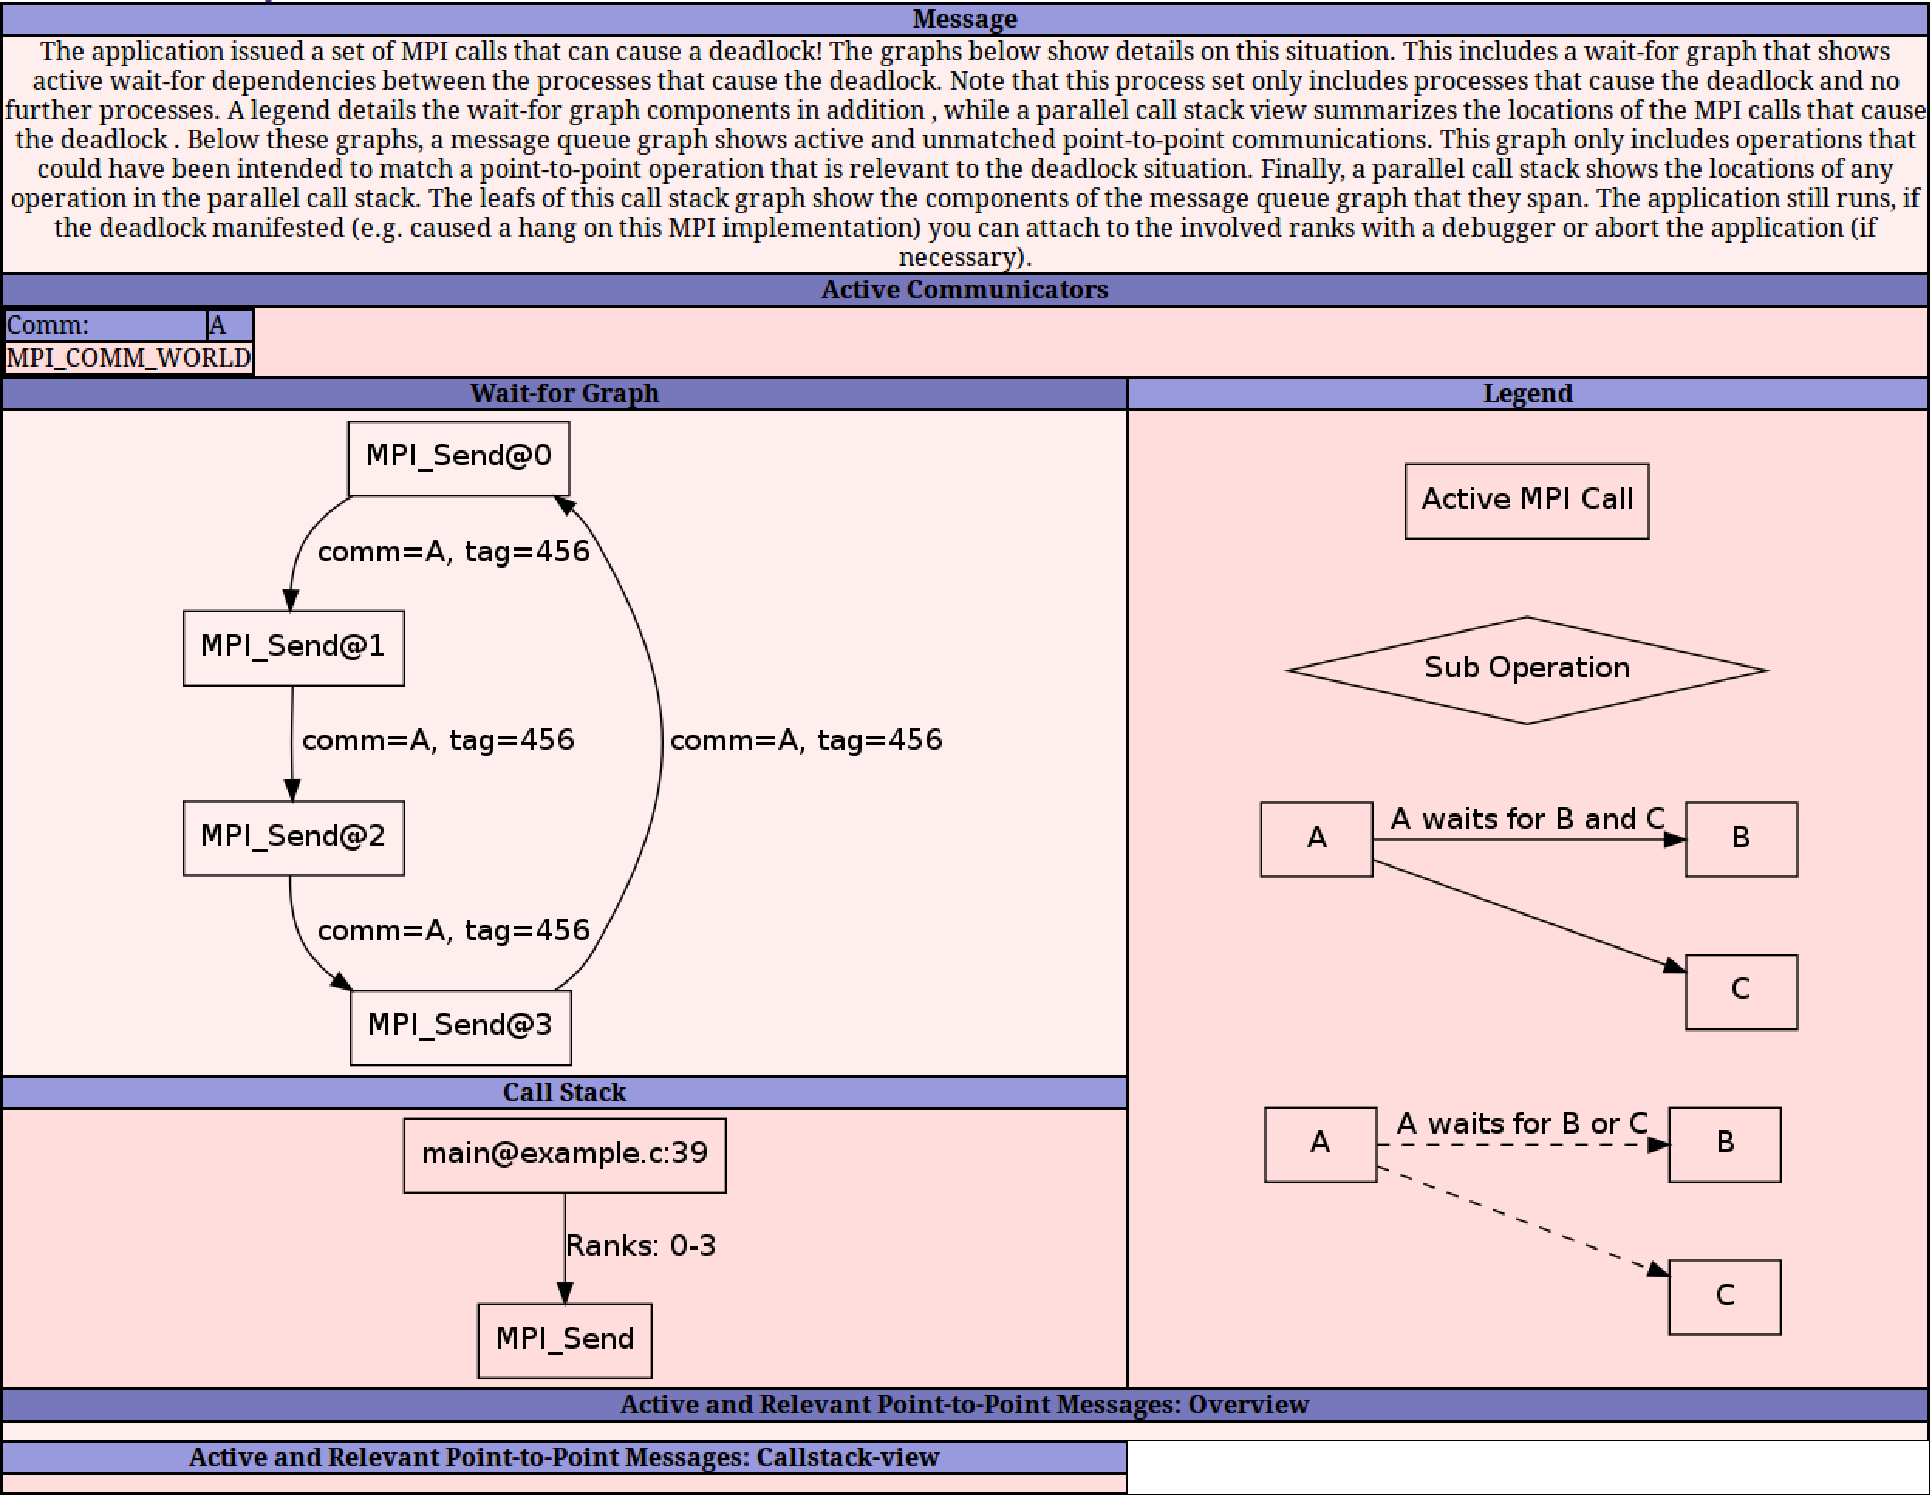
\includegraphics[angle=0,width=0.99\linewidth]{deadlock.pdf}
  \caption{Deadlock view for the send-send deadlock.}
  \label{result-deadlock-dot}
\end{figure}

% \begin{table}[hbtp]
% \begin{longtable}[t]{|m{0.05\textwidth}|m{0.06\textwidth}|m{0.38\textwidth}|m{0.14\textwidth}|m{0.23\textwidth}|}
% 
%     \multicolumn{5}{p{\textwidth}}{\textbf{MUST Output}, date: Thu Aug 25 09:04:01 2011.}\\\hline
%         \footnotesize\cellcolor{MustBlue1}\begin{center}\textbf{Rank} \end{center}&
%         \footnotesize\cellcolor{MustBlue2}\begin{center}\textbf{Type} \end{center}&
%         \footnotesize\cellcolor{MustBlue1}\begin{center}\textbf{Message} \end{center}&
%         \footnotesize\cellcolor{MustBlue2}\begin{center}\textbf{Form} \end{center}&
%         \footnotesize\cellcolor{MustBlue1}\begin{center}\textbf{References} \end{center}\\\hline
% 
%         \footnotesize\cellcolor{MustRedDark}&
%         \footnotesize\cellcolor{MustRedLight}\begin{center}\textbf{Error}\end{center}&
%         \footnotesize\cellcolor{MustRedDark}\begin{center}The application issued a set of MPI calls that can cause a deadlock! A graphical representation of this situation is available in the file named "MUST\_Deadlock.dot". Use the dot tool of the graphviz package to visualize it, e.g. issue "dot -Tps MUST\_Deadlock.dot -o deadlock.ps". The graph shows the nodes that form the root cause of the deadlock, any other active MPI calls have been removed. A legend is available in the dot format in the file named "MUST\_DeadlockLegend.dot", further information on these graphs is available in the MUST manual. References 1-4 list the involved calls (limited to the first 5 calls, further calls may be involved). The application still runs, if the deadlock manifested (e.g. caused a hang on this MPI implementation) you can attach to the involved ranks with a debugger.\end{center}&
%         \footnotesize\cellcolor{MustRedLight}&
%         \footnotesize\cellcolor{MustRedDark}\begin{center}reference 1: call\newline MPI\_Send@rank 0\newline
% reference 2: call\newline MPI\_Send@rank 1\newline
% reference 3: call\newline MPI\_Send@rank 2\newline
% reference 4: call\newline MPI\_Send@rank 3 \end{center}\\
% \hline
% \end{longtable}
% \caption{Send-send deadlock report from MUST.}
% \label{result-deadlock}
% \centering
% \end{table}

The second error results from the application calling send calls that can lead
to deadlock (Figure~\ref{result-deadlock}). Each task issues one call to
\texttt{MPI\_Send} while no matching receive is available. This can cause
deadlock, however, as such calls would be buffered for most MPI implementations this is a deadlock that only manifests
for some message sizes or MPI implementations. 
 
% \begin{figure}[hbtp]
% 	\centering
%     \subfigure[Wait-for
%     graph.]{\centering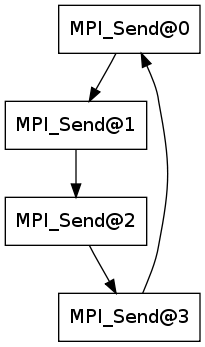
\includegraphics[width=0.25\textwidth]{deadlock.png}}
%     \subfigure[Legend]{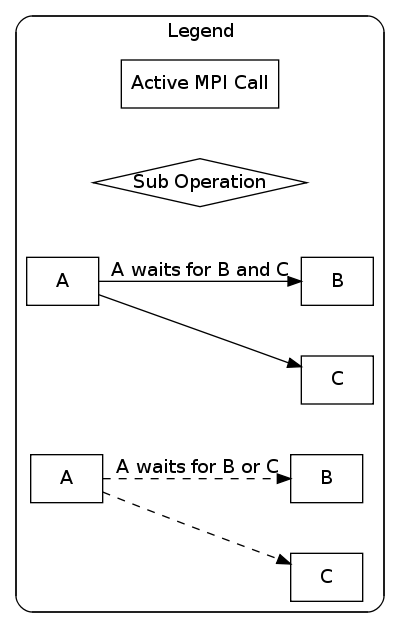
\includegraphics[width=0.45\textwidth]{deadlockLegend.png}}
%     \caption{Visualization of the send-send deadlock from
%     Table~\ref{result-deadlock}.}
%     \label{figure-deadlock}
% \end{figure}

If MUST detects a deadlock it provides a visualization for its core, i.e. the
set of MPI calls of which at least one call has to be modified or replaced.
It stores a wait-for graph representation of this core in a file named
\emph{MUST\_Deadlock.dot}. 
If available, MUST automatically translates this file into an image and provides
a deadlock view (Figure~\ref{result-deadlock-dot}), which shows the task
dependencies and a parallel call stack.
This graph file uses the DOT language of the
\emph{Graphviz} package. 
If a graphviz installation was available when
MUST was installed, it automatically visualizes the
graph, otherwise you can visualize it by issuing \emph{dot -Tps
MUST\_Deadlock.dot -o deadlock.ps} after installing this tool.
You can open the file \emph{deadlock.ps} with the post
script viewer of your choice (DOT also supports additional output formats).
If MUST was
configured with Dyninst (Section~\ref{section:dyninst}), it will also print a
parallel call stack in a file called \emph{MUST\_DeadlockCallStack.dot}, which
Figure~\ref{result-deadlock-dot} shows at the bottom. This stack includes any
MPI call that was referred to in the wait-for graph. Especially if processes use
non-blocking communications, this call stack may include multiple MPI calls for
each process.

Further graphs in the deadlock view show information about the message
matching state to highlight any call that might have been intended to match a
blocked point-to-point call. Since no outstanding point-to-point message exists
in the deadlock situation of Figure~\ref{result-deadlock}, these graphs are
empty.

\begin{figure}[t]
  \centering
  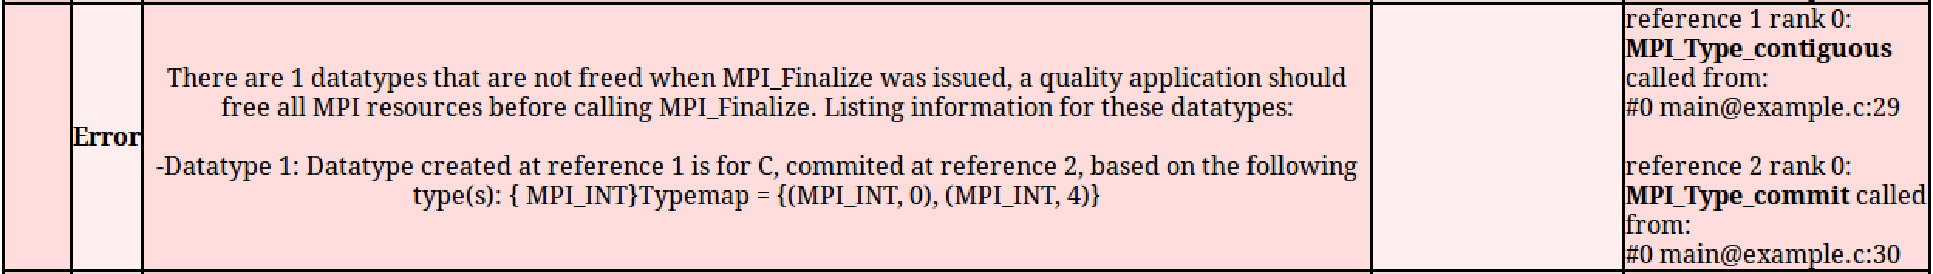
\includegraphics[angle=0,width=0.99\linewidth]{resleak.pdf}
  \caption{Resource leak report from MUST.}
  \label{result-leak}
\end{figure}
%\begin{table}[hbtp]
%\begin{longtable}[t]{|m{0.05\textwidth}|m{0.06\textwidth}|m{0.38\textwidth}|m{0.14\textwidth}|m{0.23\textwidth}|}
%
%     \multicolumn{5}{p{\textwidth}}{\textbf{MUST Output}, date: Thu Aug 25 09:04:01 2011.}\\\hline
%         \footnotesize\cellcolor{MustBlue1}\begin{center}\textbf{Rank} \end{center}&
%         \footnotesize\cellcolor{MustBlue2}\begin{center}\textbf{Type} \end{center}&
%         \footnotesize\cellcolor{MustBlue1}\begin{center}\textbf{Message} \end{center}&
%         \footnotesize\cellcolor{MustBlue2}\begin{center}\textbf{Form} \end{center}&
%         \footnotesize\cellcolor{MustBlue1}\begin{center}\textbf{References} \end{center}\\\hline
% 
%         \footnotesize\cellcolor{MustRedDark}&
%         \footnotesize\cellcolor{MustRedLight}\begin{center}\textbf{Error}\end{center} &
%         \footnotesize\cellcolor{MustRedDark}\begin{center}There are 1 datatypes that are not freed when MPI\_Finalize was issued, a quality application should free all MPI resources before calling MPI\_Finalize. Listing  information for these datatypes:\newline\newline
% -Datatype 1: Datatype created at reference 1 is for C, commited at reference 2, based on the following type(s): MPI\_INT  \end{center}&
%         \footnotesize\cellcolor{MustRedLight}&
%         \footnotesize\cellcolor{MustRedDark}\begin{center}reference 1: call\newline MPI\_Type\_contiguous @rank 0\newline
% reference 2: call\newline MPI\_Type\_commit @rank 0\end{center}\\
% \hline
% \end{longtable}
% \caption{Resource leak report from MUST.}
% \label{result-leak}
% \centering
% \end{table}

Finally, MUST detects that the application leaks MPI resources when calling
\texttt{MPI\_Finalize}. In particular
this is a datatype created with an \texttt{MPI\_contiguous} call. Applications
should free all such resources before invoking \texttt{MPI\_Finalize}, as
harmful leaks are easier to detect
in such cases.

\section{MUST's Operation Modes}
\label{section:must-modes}

MUST's analysis of all MPI calls causes runtime overhead. As a result, it is
important to adapt its configuration such that its overhead stays acceptable.
While its default configuration (\emph{mustrun} without additional switches) is
easy to use, more advanced configurations may be required. MUST's overhead
primarily results from:
\begin{itemize}
  \item Correctness checks that require information from multiple processes, and
  \item A communication mode that allows MUST to detect MPI usage errors even if
  the application crashes. 
\end{itemize}

MUST can use more than one additional process to run expensive correctness
checks, while a shared memory based communication mode allows MUST to tolerate
application crashs with limited runtime overhead.

\subsection{Mode Overview}

MUST provides the following operation modes that adapt its overhead to the
target use-case:
\begin{enumerate}
  \item \textbf{(Default) Very slow, Centralized, application may crash:}
  \begin{itemize}
    \item Command line: \emph{mustrun \mbox{-np X} exe}
    \item One extra process for correctness checking
    \item All checks enabled
    \item Detects errors even if application crashs
    \item Very slow, for short running tests at $<32$ processes
  \end{itemize}
  \item \textbf{Fast, centralized, application does not crash:}
  \begin{itemize}
    \item Command line: \emph{mustrun \mbox{-np X} \mbox{-{}-must:nocrash} exe}
    \item One extra process for correctness checking
    \item All checks enabled
    \item Detects errors only if the application does not crash %(but is
    %allowed to hang)
    \item Limited scalability, use for $<100$ processes 
  \end{itemize}
  \item \textbf{Fast, centralized, application may crash:}
  \begin{itemize}
    \item Command line: \emph{mustrun \mbox{-np X} \mbox{-{}-must:nodesize Y} exe}
    \item Number of extra processes: $1+\lceil{}\frac{X}{Y-1}\rceil{}$
    \item All checks enabled
    \item Detects errors even if application crashs
    \item Limited scalability, use for $<100$ processes
    \item Requires shared memory communication (Available on most linux based
    clusters) 
  \end{itemize}
  \item \textbf{Distributed, application does not crash:}
  \begin{itemize}
    \item Command line: \emph{mustrun \mbox{-np X} \mbox{-{}-must:distributed} [\mbox{-{}-must:fanin Z}] exe}
    \item Network of extra processes:
    \begin{itemize}
      \item Layer $0$: $A=\lceil{}\frac{X}{Z}\rceil{}$
      \item Layer $1$: $B=\lceil{}\frac{A}{Z}\rceil{}$
      \item \ldots
      \item Layer $k$: 1
    \end{itemize}
    \item If you need to reduce overheads, you can disable MUST's distributed deadlock detection with \emph{\mbox{-{}-must:nodl}}
    \item Detects errors only if the application does not crash %(but is
    %allowed to hang)
    \item Tested with $16,384$ processes 
  \end{itemize}
  \item \textbf{Distributed, application may crash:}
  \begin{itemize}
    \item Command line: \\\emph{mustrun \mbox{-np X} \mbox{-{}-must:distributed} \mbox{-{}-must:nodesize Y} [\mbox{-{}-must:fanin Z}] exe}
    \item Network of extra processes:
    \begin{itemize}
      \item Layer $0$: $A=\lceil{}\frac{X}{Y-1}\rceil{}$
      \item Layer $1$: $B=\lceil{}\frac{A}{Z}\rceil{}$
      \item Layer $2$: $C=\lceil{}\frac{B}{Z}\rceil{}$
      \item \ldots
      \item Layer $k$: 1
    \end{itemize}
    \item If you need to reduce overheads, you can disable MUST's distributed deadlock detection with \emph{\mbox{-{}-must:nodl}}
    \item Tested with $4,096$ processes 
    \item Requires shared memory communication (Available on most linux based clusters)
  \end{itemize}
\end{enumerate} 

\subsection{Mode Details}

For any non-demanding (short and small scale) use-case we suggest operation 
Mode~1 (\emph{mustrun \mbox{-np X} exe}), since it is always available and easy to use.

For more extensive application runs at moderate scale ($<100$ processes) users
should either use Mode~2 (\emph{mustrun \mbox{-np X} \mbox{-{}-must:nocrash} exe}) or Mode~3
(\emph{mustrun \mbox{-np X} \mbox{-{}-must:nodesize Y} exe}). While Mode~2 assumes that the
application does not crash, Mode~3 uses a shared memory communication (Linux
message queues) to tolerate application crashs. Besides the limited availability
of this communication mechanism (most linux based systems), it requires more
than one extra process to operate. The user needs to specify a nodesize $Y$ that
is a divisor of the number of cores available within each compute node. MUST
then uses one tool process per $Y-1$ application processes. It is important that
the resource manager distributes MPI ranks in node-core order. That is, it fills
each node completely and with successive ranks. The use of the
\emph{\mbox{-{}-must:fillnodes}} switch to the \emph{mustrun} command may help if the
total number of MPI ranks does not fill all allocated nodes causing the
resource manager to not fill nodes completely.

By adding the \emph{\mbox{-{}-must:info}} switch to any \emph{mustrun} command, the user
may retrieve additional information on the number of application tasks, tool
tasks, and required nodes without running or preparing a MUST run. This provides
valuable information to prepare batch job allocations.

Modes~4 (\emph{mustrun \mbox{-np X} \mbox{-{}-must:distributed} [\mbox{-{}-must:fanin Z}] exe}) and 5
(\emph{mustrun \mbox{-np X} \mbox{-{}-must:distributed} \mbox{-{}-must:nodesize Y} [\mbox{-{}-must:fanin Z}] exe})
are intended for application runs at scale ($>100$ processes, where we
tested MUST with up to $16{,}384$ processes). Both modes use a tree network to
run several correctness checks, which increase their demand for extra computing
cores. Again Mode~4 assumes that the application does not crash, while Mode~5
uses a shared memory communication to tolerate application crashs. Mode~5 comes
with the same restrictions and allocation assumptions as Mode~3. For
both modes, the user may specify the \emph{\mbox{-{}-must:fanin Z}} switch which
controls the ratio of application to extra tool processes. The default
value is $16$, higher values may increase MUST's overhead, while lower
values may reduce its overhead. Experience with MUST's
distributed deadlock detection shows that it
scales to an order of $16{,}384$ processes, but can double
MUST's overhead. 
If MUST's overhead is too high for your use-case, you can add the switch
\emph{\mbox{-{}-must:nodl}} to disable the distributed deadlock detection for Modes~4 and~5. 

\section{Included Checks}
MUST currently provides correctness checks for the following classes of errors:
\begin{itemize}
  \item Constants and integer values
  \item Communicator usage
  \item Datatype usage
  \item Group usage
  \item Operation usage
  \item Request usage
  \item Leak checks (MPI resources not freed before
  calling \texttt{MPI\_Finalize})
  \item Type mis-matches
  \item Overlapping buffers passed to MPI
  \item Deadlocks resulting from MPI calls
\end{itemize}

\section{Optional: MUST Installation with Dyninst}
\label{section:dyninst}
In order to install MUST with Dyninst support a full Dyninst installation or a
separate installation of the Dyninst Stackwalker API is needed. This usually
requires an installation of libdwarf. Installation instructions for these can be
found on the Dyninst website\footnote{http://www.dyninst.org/}. We tested the integration of 
dyninst in versions 7.0.1 and 8.0.1 and stackwalkerAPI in versions 2.1 and 8.0.1.
For some systems we identified issues for the older version of dyninst, 
that are listed in Section \ref{subsect:dyninst-issues}. 
We suggest to
install libdwarf as a shared library (\emph{\mbox{-{}-}enable-shared} during its
configure).

As Dyninst's build support is currently limited to GNU compilers, you should 
build your application and the tool with binary compatible compilers. 
To build dyninst 
with compilers other than GNU, make sure to set the variables \emph{CC}, \emph{CXX}, 
\emph{GXX}, \emph{LD} and \emph{LINKER} for both, the configure and the make step 
(this is not supported).

After a successful installation of the Stackwalker API it is necessary
to configure MUST to use this installation. Use the following CMake variables:
\begin{itemize}
  \item \textbf{-DUSE\_CALLPATH=On} Enables the feature
  \item \textbf{-DSTACKWALKER\_INSTALL\_PREFIX=} Should point to the 
  directory used for Stackwalker API installation (i.e. prefix given to its
  configure)
  \item \textbf{-DCALLPATH\_STACKWALKER\_EXTRA\_LIBRARIES=} Additional libaries
  that are needed, if libdwarf was built statically you will need to add an
  absolute filepath to this lib here
\end{itemize}

Afterwards run \emph{make} and \emph{make install} to build and install MUST.
When running MUST no additional steps are needed. However, the stackwalker
library will only be able to extract source file names and line numbers if the
application was built with the debugging flag \emph{-g}. Otherwise, it will list
symbol addresses and library names instead.

Note that MUST expects that the shared libraries for libdwarf (if built as a shared library) 
and libelf are in the \texttt{LD\_LIBRARY\_PATH}.

\section{Troubleshooting}

The following lists currently known problems or issues and potential
workarounds.

\subsection{Issues with Ld-Preload}
In order to use MUST, your application must be linked against the core library of
\pnmpi. Per default MUST will add this library at execution time by using the
ld-preload mechanism. If this causes issues you can use the following
command to manually link the \pnmpi library:
\begin{verbatim}
mpicc source.c -L<PNMPI-INSTALLATION-DIR>/lib  \
        -lpnmpi -o application.exe
\end{verbatim}

Important: if you manually link against the MPI library, you must add the \pnmpi
library first and the MPI library afterwards.

\subsection{Issues with stackwalkerAPI}
\label{subsect:dyninst-issues}

\paragraph{boost related error while build of MUST with dyninst-8:}
\begin{verbatim}
error: boost/bar_foo.hpp: File not found
\end{verbatim}
Solution for boost installation outside of /usr:

Edit \emph{mustsrc/modules/Callpath/CMakeLists.txt} insert around line 21:
\begin{verbatim}
include_directories(/<BOOST_INSTALL_PREFIX>/include)
\end{verbatim}

\paragraph{SEGFAULT on execution of \emph{mustrun}:}
\begin{verbatim}
  rank 0 (of 4), pid 12345 catched signal nr 11
\end{verbatim}
without any of the WARNINGs listed below. This issue affects almost every installation.\newline\newline
Solution:

Edit \emph{src/dyninst/symtabAPI/src/Object-elf.C} around line 2069 and replace:
\begin{verbatim}
  if(secNumber >= 1 && secNumber <= regions_.size()) {
\end{verbatim}
by
\begin{verbatim}
  if(secNumber >= 0 && secNumber < regions_.size()) {
\end{verbatim}
... and rebuild / install dyninst

\paragraph{SEGFAULT on execution of \emph{mustrun}:}
\begin{verbatim}
  rank 0 (of 4), pid 12345 catched signal nr 11
\end{verbatim}
without any of the WARNINGs listed below and after fixing the issue above.\newline\newline
Solution:

Make sure that you use the same compiler family for building dyninst, \pnmpi, 
GTI, MUST and your application!

\paragraph{\emph{mustrun} reports missing library:}

\begin{verbatim}
  WARNING: Can't load module libcallpathModule.so (Error libdwarf.so: 
  cannot open shared object file: No such file or directory)
\end{verbatim}
Solution:

Add \emph{\textless LIBDWARF\mbox{--}INSTALLATION\mbox{--}DIR\textgreater/lib} to 
\emph{LD\_LIBRARY\_PATH} (\emph{libdwarf.so} should be located there).


\section{Copyright and Contact}
MUST is distributed under a BSD style license, for details see the file
\mbox{LICENSE.txt} in its package. MUST uses parts of external code, mostly distributed 
under BSD style license, in any case the license is indicated in the source file and in 
the external directories, a LICENSE file can be found.
Finally, \pnmpi is distributed under LGPL license. The license file is located in 
\mbox{externals/GTI/externals/PnMPI/LICENSE}.


Contact \emph{must-feedback@lists.rwth-aachen.de} for bug reports, feedback, and
feature requests.

\end{document}
